\documentclass[11pt]{article}
\usepackage{amsmath, mathtools, amsthm, graphicx, float, bm}

\DeclareMathOperator{\di}{d\!}

\newcommand{\Unif}{\textit{Unif}[0,1]}

\newtheorem{proposition}{Proposition}

\begin{document}
\title{Diversity Incentives for Recruiters}
\author{Prasanna Parasurama}
\date{\today}
\maketitle

\begin{abstract}
    This paper concerns the effectiveness of diversity incentives for recruiters. I address whether incentives for recruiters to source diverse candidates is effective in increasing the diversity of the workforce. I first develop a theoretical model --  a 2-stage hiring game in which, recruiters are incentivized to shortlist the best candidates with an additional bonus for diverse candidates, and managers are incentivized to hire the best candidate from the shortlist -- and solve this model under expected utility theory. Second, I propose an experiment to test whether the empirics align with the theoretical predictions, and test whether behavioral concerns such as stereotyping play a role.
\end{abstract}

\section{Introduction}
Underrepresentation of women and minorities in the STEM labor force has far reaching social and economic implications from untapped innovative capabilities to economic inequality.
Organizations have attempted to address this issue in a multitude of ways: disclosing diversity reports, employing Diversity and Inclusion officers, and instituting policies to increase workforce diversity. One such policy is an incentive scheme for recruiters to source and recruit diverse candidates. Around 2015, Facebook implemented a point system in which recruiters get 1 point for every new hire and an additional point if the new hire is diverse. Recently, however, doubts have been raised about the effectiveness of this policy due to the misalignment of incentives between recruiters and engineers/managers, who ultimately make the hiring decision. Often, managers' compensation are directly tied to team performance and do not get extra incentives to hire diverse candidates. The reporter in the Bloomberg article writes:

``The recruiters saw that many of their diversity candidates didn’t end up getting an offer. Two former recruiters blamed in part the engineering department’s candidate review process, a twice- or thrice-weekly meeting at which every engineering offer had to be approved''

Similar phenomenon have been pointed out by researchers. For example, in a research paper that studies the effects founder experience and gender on hireablity, a recruiter interviewed by the auothers is quoted:

“A technical recruiter at a search firm (Recruiter 16) who noted that “tons of companies come to us because all they want is diversity candidates” also stated that his clients are interviewing a lot of diversity candidates but not hiring them at the same rate” (Botelho and Chang 2019).

This raises an important question of whether policies that incentivize recruiters, but not managers, to recruit diverse candidates are effective in increasing the diversity of the workforce, let alone not be counterproductive. I address this question in what follows.

\section{Literature}


\section{Theoretical Model and Predictions}

\subsection{Model}

I model the hiring process as a 2-stage game.
In the first stage, the recruiter receives applications from $n_a$ candidates, of which $n_m$ are male and $n_f$ are female. Each candidate has productivity $q$, which is a random variable drawn from a distribution with cumulative distribution function $F_q(\cdot)$ and density function $f_q(\cdot)$. Even though the recruiter doesn't observe the true productivity $q$, he\footnote{I will use the pronouns ``he'' and ``she'' to refer to the recruiter and the hiring manager respectively.} observes a noisy signal of productivity, $\hat{q_r}$, which is correlated with the true productivity -- this is akin to recruiters inferring applicants' productivity from resumes, for example.
The recruiter's task is to shortlist $n_s$ candidates to send to the manager. He receives a payout that is proportional to the quality of the candidate hired by the manager ($c_rq$), and receives an additional diversity bonus, if the hired candidate is female ($c_rq + bq$). Formally, the recruiter's utility function is:

\[  U_r =
    \begin{cases}
        c_rq     & \textit{if male is hired}          \\
        (b+c_r)q & \textit{if female is hired}, b > 0
    \end{cases}
\]

In the second stage of the game, the hiring manager receives $n_s$ shortlisted candidates from the recruiter. Like the recruiter, the manager also has her own assessment of the candidates productivty $\hat{q}_h$, and her task is to hire $n_h$ candidates. The manager receives a payout that is proportional to the applicant's true quality $q$, but receives no additional bonus for hiring a female candidate. The manager's utility function is thus:

$$U_h = c_hq$$

\begin{center}
    \begin{tabular}{ l l}
        \hline
        Symbol     & Definition                                          \\
        \hline
        $F(\cdot)$ & Cumulative distribution function                    \\
        $f(\cdot)$ & Probability density function                        \\
        $q$        & Candidate's productivity                            \\
        $m$        & Male                                                \\
        $f$        & Female                                              \\
        $c_r$      & Recruiter's commission                              \\
        $b$        & Recruiter's diversity bonus                         \\
        $c_h$      & Hiring Manager's commission                         \\
        $U_r$      & Recruiter's utility                                 \\
        $S$        & Recruiter's expected utility under optimal decision \\
        $U_h$      & Hiring manager's utility                            \\
    \end{tabular}
\end{center}

\subsection{Theoretical Predictions}

In this section, I simplify the above model by fixing some parameters, and solve the simplified model under expected utility theory. This will serve as a baseline comparison for experimental results.

Assume that the true productivity of both male and female candidates are identically distributed under $\textit{Unif}[0,1]$, and that this is common knowledge.
The recruiter's task is to send 2 candidates to the manager. However, for mathematical simplicity, instead of shortlisting 2 candidates in the same round, the recruiter shortlists 2 candidates in 2 rounds -- that is, he shortlists 1 candidate in a round, and shortlists another in the subsequent round. The manager receives 2 candidates in total (from 2 rounds), and her task is to hire 1 candidate.

Without loss of generality, further assume that the recruiter's and manager's commissions are both 1, $c_r=c_h=1$. For brevity, redefine $b$ so that $b>1$. That is, Instead of writing $U_{r,f} = (1+b)q, b>0$  we write $U_{r,f} = bq, b>1$.

\begin{align*}
     & q \sim \textit{Unif}[0,1] \\
     & U_r =
    \begin{cases}
        q  & \textit{if male is hired}        \\
        bq & \textit{if female is hired}, b>1
    \end{cases}    \\
     & U_h = q
\end{align*}

In each round, given there are $n_m$ male candidates and $n_f$ female candidates in a set of candidates $k=\{k_1, k_2...k_{n_m+n_f}\}$, with corresponding productivies $\{q_1...q_{n_m+n_f}\}$ and utilities  $\{U(k_1)...(U(k_{n_m+n_f}))\}$, the recruiter will shortlist a candidate that will maximize his expected utility -- Note that this utility is a function of the candidate's productivity, gender $g$ of the candidate, as well as the diversity bonus.
$$S \equiv \max_k U_r(q, b, \textit{gender})$$

Likewise, given a set of shortlisted candidates $l=\{l_1...l_{n_l}\}$ manager will hire a candidate that maximizes her own expected utility, which is only a function of the candidate's productivity.

$$\max_l U_h(q)$$


\begin{proposition}
    The probability that a male is shortlisted decreases with bonus $b$.
\end{proposition}

\begin{proof}
    Given the productivies of male and female candidates are uniformly distributed, the recruiter's utility from male and female candidates are also uniformly distributed:
    \begin{align*}
         & U_{r,m} \sim Unif[0,1] \\
         & U_{r,f} \sim Unif[0,b]
    \end{align*}

    Let $S_m$ and $S_f$ be the maximum utility to be gained from male and female candidate respectively:
    $S_m=Max(U_{r_m})$ and $S_f=Max(U_{r_f})$. Note that $S_m$ and $S_f$ are $n^{th}$ order statistic of a uniform distribution, with the following CDFs:

    \begin{align*}
         & F_{S_m}(x) =
        \begin{cases}
            x^{n_m} & 0 < x < 1 \\
            1       & x \geq 1  \\
            0       & otherwise
        \end{cases}
        \\
         & F_{S_f}(x) =
        \begin{cases}
            \frac{x}{1+b}^{n_f} & 0 < x < 1+b  \\
            1                   & x \geq 1 + B \\
            0                   & otherwise
        \end{cases}
    \end{align*}


    A male candidate is shortlisted when the maximum utility gained from a male candidate exceeds the maximum utility gained from a female candidate: $S_m=Max(U_{r_m}) > S_f=Max(U_{r_f})$. Then, the probaility that a male is shortlisted is:
    \begin{align*}
        Pr(S_m > S_f) & = Pr(S_f = x) Pr(S_m > x)                        \\
                      & = \int_{0}^{b+1} f_{S_m}(x) (1-F_{S_f}(x)) \di x \\
                      & = \frac{(b+1)^{-n_f} n_m}{n_f+n_m}
    \end{align*}

    Since $n_m, n_f >0$, the above expression is decreasing with bonus $b$.

\end{proof}

\begin{proposition}\label{prop_male_exp_qual}
    The expected produtivity of shortlisted male candidates is independent of bonus $b$.
\end{proposition}
\begin{proof}
    Consider the conditional density function of the recruiter's utility from a male candidate that is shortlisted --  $f_{S_m|S_m>S_y}$. This conditional density function can be written as:

    \begin{align*}
        f_{S_m|S_m>S_f}(x) & = \frac{f_{S_m}(x)F_{S_f}(x) }{Pr(S_m > S_f)}     \\
                           & = \frac{(n_f+n_m)(x^{n_f+n_m-1})}{n_mBeta[n_m,1]}
    \end{align*}

    Expected utility from a shortlisted male candidate is then:

    \begin{align*}
        E[S_m|S_m > S_y] & = \int_0^1{xf_{S_m|S_m>S_y}(x) \di x} \\
                         & = \frac{n_m + n_f}{1+n_f+n_m}
    \end{align*}

    Since $U_r = q$ for male candidates:

    $$E[q_m|S_m > S_y] = \frac{n_m + n_f}{1+n_f+n_m}$$

    which is independent of bouns $b$.
\end{proof}


\begin{proposition}\label{prop_female_exp_qual}
    The expected produtivity of shortlisted female candidates decreases with bonus $b$
\end{proposition}
\begin{proof}
    Following the proof of Proposition \ref{prop_male_shortlist_productivity}, the conditional density function of the recruiter's utility of a shortlisted female candidate is

    \begin{align*}
        f_{S_f|S_f>S_m}(x) & = \frac{f_{S_f}(x)F_{S_m}(x) }{Pr(S_f > S_m)} \\
                           & = \begin{cases}
            \frac{n_f(n_f+n_m)x^{(n_f-1)}x^{n_m}}{-n_m+b^{n_f}(n_f+n_m)} & 0 \leq x < 1    \\
            \frac{n_f(n_f+n_m)x^{(n_f-1)}}{-n_m+b^{n_f}(n_f+n_m)}        & 1 \leq x \leq b \\
        \end{cases}
    \end{align*}

    The expectation of the recruiter's utility from a shortflisted female candidate is:

    \begin{align*}
        E[S_f|S_f > S_m] & = \int_0^1{x \frac{ n_f(n_f+n_m)x^{(n_f-1)}x^{n_m}}{-n_m+b^{n_f}(n_f+n_m)} \di x}                 \\
                         & + \int_1^b{x \frac{n_f(n_f+n_m)x^{(n_f-1)}}{-n_m+b^{n_f}(n_f+n_m)} \di x}                         \\
                         & = \frac{n_f(n_f+n_m)(-n_m+b^{(1+n_f)} (1+n_f+n_m))}{(1+n_f) (1+n_f+n_m) (-n_m+b^{n_f} (n_f+n_m))}
    \end{align*}

    Since the recruiter's utility is $U_r = bq \implies q = \frac{U_r}{b}$ for female candidates,
    \begin{align*}
        E[q_f|S_f > S_m] & = \frac{1}{b} \frac{n_f(n_f+n_m)(-n_m+b^{(1+n_f)} (1+n_f+n_m))} {(1+n_f) (1+n_f+n_m) (-n_m+b^{n_f} (n_f+n_m))}
    \end{align*}

    Taking the derivative of the above expression with respect to $b$:
    \begin{align*}
         & \frac{\di E[q_f|S_f > S_m]} {\di b}  =                                                                                                                             \\
         & - \frac{[n_f n_m (n_f+n_m)] [\left(-(n_f+1) b^{n_f} (n_f+n_m)+n_f b^{n_f+1} (n_f+n_m+1)+n_m\right)]}{b^2 (n_f+1) (n_f+n_m+1) \left(n_m-b^{n_f} (n_f+n_m)\right)^2}
    \end{align*}

    Note that the two terms in the numerator and the term on the denominator are positive for $n_m, n_f \geq 1, b>1$, making the whole term negative.

\end{proof}

\begin{proposition}
    Given a shortlist of a male and a female, the probability that a male is hired increases with bonus $b$, and the probability that a female is hired decreases with bonus $b$.
\end{proposition}

\begin{proof}
    The intuition for this proposition is as follows: bonus $b$ changes the quality distribution of a shortlisted female, which in turn affects the conditional probability that a male is hired. As bonus $b$ increases, the expected quality of a shortlisted female decreases (proposition \ref{prop_female_exp_qual}), however the expected quality of a shortlisted male remains the same \ref{prop_male_exp_qual}. As a result, the conditional probability that a male is hired increases.

    Formally, consider the conditional probability that a male is hired given a shortlist $\bm{s}=\{m,f\}$ (i.e. one male, one female), and define it as $Pr(n_{h_m}=1|\bm{s}=\{m,f\})$ This is the probability that the quality of the shortlisted male exceeds the quality of the shortlisted female:
    \begin{align*}
        Pr(\textit{Male is hired}|\bm{s}=\{m,f\}) & \equiv Pr(n_{h_m}=1|\bm{s}=\{m,f\})     \\
                                                  & = Pr([q_m|S_m > S_f] > [q_f|S_f > S_m])
    \end{align*}

    where $q_m|S_m > S_f$ and $q_f|S_f > S_m$ are the qualities of shortlisted male and female respectively. From Proposition \ref{prop_male_exp_qual}, we know the distribution of the recruiter's utility from a shortlisted male. Because the recruiter's utility equals the quality for male candidates ($U_{r,m} = q$), quality of shortlisted male follows the same distribution as the recruiter's utility.

    \begin{align*}
        f_{q_m|S_m > S_y} = f_{S_m|S_m > S_y} = \frac{(n_f+n_m)(x^{n_f+n_m-1})}{n_mBeta[n_m,1]}
    \end{align*}

    For female candidates, we know the distribution of the recruiter's utility from a shortlisted female candidate. Using the change of variable technique with respect to the function $g: U_{r,f} = bq$, we can get the quality distribution of a shortlisted female.

    \begin{align*}
        f_{q_f|S_f > S_m}(x) & = f_{S_f|S_f > S_m} (g^{-1}(x)) \lvert \frac{\di}{\di x} (g^{-1}(x)) \rvert \\
                             & = \frac{n_f (n_f+n_m) x^{n_f-1} \left(
            \begin{array}{cc}
                     &
                    \begin{array}{cc}
                        x^{n_m} & 0<x<1   \\
                        1       & x\geq 1 \\
                    \end{array}
                    \\
                \end{array}
            \right)}{b^{n_f} (n_f+n_m)-n_m}
    \end{align*}

    Using these two distributions:

    \begin{align*}
         & Pr(n_{h_m=1}|bm{s}=\{m,f\})                                                                                                                             \\
         & = Pr([q_m|S_m > S_f] > [q_f|S_f > S_m])                                                                                                                 \\
         & = \int_{0}^{b+1} f_{q_m|S_m > S_f}(x) (1-F_{q_f|S_f > S_m}(x)) \di x                                                                                    \\
         & = \frac{b^{-n_f-n_m} \left(-2 n_m (2 n_f+n_m) b^{n_f+n_m}+2 (n_f+n_m)^2 b^{2 n_f+n_m}+n_f n_m\right)}{2 (2 n_f+n_m) \left(b^{n_f} (n_f+n_m)-n_m\right)}
    \end{align*}

    Taking the derivative of the above expression w.r.t $b$:
    \begin{align*}
         & \frac{\di}{\di b} Pr(n_{h_m=1}|bm{s}=\{m,f\})                                                                                                             \\
         & = \frac{n_f n_m (n_f+n_m) b^{-n_f-n_m-1} \left(b^{n_f} (-(2 n_f+n_m))+2 n_f b^{2 n_f+n_m}+n_m\right)}{2 (2 n_f+n_m) \left(n_m-b^{n_f} (n_f+n_m)\right)^2}
    \end{align*}

    which is positive for $b, n_m, n_f \geq 1$.

\end{proof}


\begin{proposition}
    The overall probability that a male is hired decreases with bonus $b$, and the overall probability that a female is hired increases with bonus $b$.
\end{proposition}

\begin{proof}
    The overall probability that a male is hired depends on both the probability that a male is shortlisted, and the probability that a male is hired given a shortlist.

    Recall that $Pr(n_{h,m}=1|\bm{s})$ is the conditional probability that a male is hired given shortlist $\bm{s}$. Further define $Pr(n_{h,m}=1)$ as the overall probability that a male is hired, and $n_{s,m}$ as the number of shortlisted males.

    \begin{align*}
         & Pr(\textit{Male is Hired}) \equiv Pr(n_{h,m}=1)                               \\
         & = \sum\nolimits_{n_{s,m} \in \{0,1,2\}} Pr(n_{h,m}=1|\bm{s}) Pr(n_{s,m})      \\
         & = Pr(n_{s,m} = 0)Pr(n_{h,m}=1|\{f,f\}) + Pr(n_{s,m} = 1)Pr(n_{h,m}=1|\{m,f\}) \\
         & \qquad + Pr(n_{s,m} = 1)Pr(n_{h,m}=2|\{m,m\})
    \end{align*}

    Note that $Pr(n_{s,m})$ has a binomial distribution with parameter $p=Pr(\text{Male is shortlisted})=\frac{(b+1)^{-n_f} n_m}{n_f+n_m}$ and $n=2$. Substituting this in:

    \begin{align*}
        Pr(n_{h,m}=1) & = \binom{2}{0}p^0(1-p)^2 Pr(n_{h,m}=1|\bm{s}) +  \binom{2}{1}p(1-p) Pr(n_{h,m}=1|\bm{s})                                           \\
                      & \qquad + \binom{2}{2}p^2(1-p)^0 Pr(n_{h,m}=1|\bm{s})                                                                               \\
                      & =  0 + \binom{2}{1}p(1-p) Pr(n_{h,m}=1|\bm{s}) + \binom{2}{2}p^2(1-p)^0                                                            \\
                      & = \frac{n_m b^{-3 n_f-n_m} \left(-n_m (2 n_f+n_m) b^{n_f+n_m}+2 (n_f+n_m)^2 b^{2 n_f+n_m}+n_f n_m\right)}{(n_f+n_m)^2 (2 n_f+n_m)}
    \end{align*}


    Taking the derivative of the above expression with respect to $b$:

    \begin{align*}
         & \frac{\di}{\di b} Pr(n_{h,m}=1) =                                                                                                         \\
         & -\frac{[n_f n_m b^{-3 n_f-n_m-1}] [-2 n_m (2 n_f+n_m) b^{n_f+n_m}+2 (n_f+n_m)^2 b^{2 n_f+n_m}+n_m (3 n_f+n_m)])}{(n_f+n_m)^2 (2 n_f+n_m)}
    \end{align*}

    Because $n_m, n_f, b \geq q$, the first term on the numerator and the denominator are always positive. Part of the second term can be written as:
    \begin{align*}
        -2 n_m (2 n_f+n_m) b^{n_f+n_m}+2 (n_f+n_m)^2 b^{2 n_f+n_m} & = \\
        2b^{2n_f+n_m} + 4b^{2n_f+n_m} n_f n_m + 2b^{2n_fn_m} m^2 - 4b^{n_fn_m}n_fn_m - 2b^{n_f+n_m}m^2
    \end{align*}

    Since $4b^{2n_f+n_m} n_f n_m > 4b^{n_fn_m}n_fn_m$ and $2b^{2n_fn_m} m^2 > 2b^{n_f+n_m}m^2$ for $n_f,n_m,b \geq 1$, the second term is also positive. This makes the derivative negative.
\end{proof}

\section{Experimental Setup}

The experiments are aimed to closely mirror the theoretical model described in section 2. Participants are recruiter on a (Mechanical Turk). Each recruiter is matched with a hiring manager, and they play 10 rounds total (10 total hires), before the participants are rematched.  Note that this is a between-subject design -- once a participant is assigned to a treatment cell, it will not change throughout the experiment. Managers and recruiters are informed of their own payment structure, as well as their counterparty's payment structure. In addition, both the managers and recruiters receive the full set of instructions, so everything below is common knowledge. \\

In each round, each recruiter receives 10 resumes (7 male, 3 female candidates)\footnotemark, which contains the candidate's name, GPA, Degree, Field of Study, and Years of Experience. The gender of the candidate is made salient by the name. Recruiters are asked to assess the candidates quality and shortlist 1 or 2 candidates for a fictional software engineering job. They are further informed that the true quality $q$ of the candidate is composed of two components: first, a deterministic quality score $q'$ that depends on the candidate's credentials (GPA, Degree, Field of Study, Yrs of Experience). They are shown a schema for how quality score $q'$ is related to credentials as well as some examples. In general, higher the GPA, Yrs of Experience, and Degree, and more technical the field of study, the higher the score. Second, there is a random error term $\epsilon$, that is added to the score. This implies that in some cases, even if a candidate has stellar credentials, their true quality may be less that stellar; but in general, better credentials mean higher quality. Recruiters are informed that the distribution of qualities among male and female candidates are the same in the initial candidate pool -- that is, on average, a male candidate has the same quality as a female candidate.


$$q = 0.7q' + 0.3\epsilon$$
$$q' = f(\textit{GPA, Degree, Field of Study, Yrs Exp})$$


\footnotetext{This reflects the actual gender proportion in software engineering jobs.}

\begin{figure} % not "pt"
    \centering
    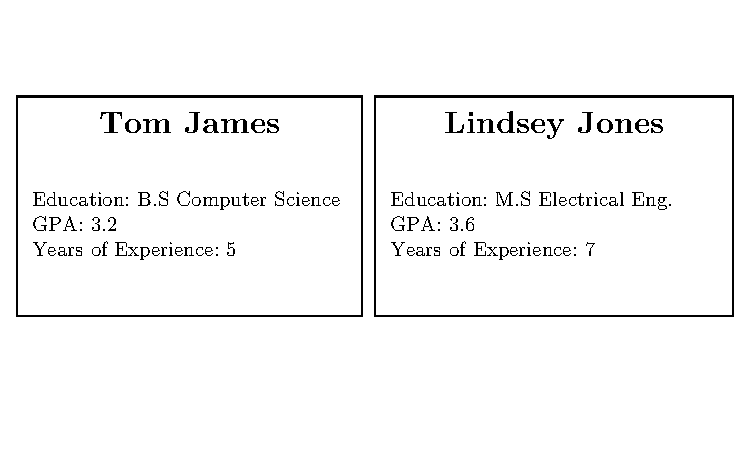
\includegraphics[width=\textwidth, keepaspectratio]{illus/resumes.pdf}
    \caption{Illustration of Resumes}
    \label{sample_resumes}
\end{figure}

Once a recruiter shortlists 2 candidates, the manager receives the resumes of the shortlisted candidates. The managers are asked to assess each candidate's quality and hire one candidate. Once the manager hires a candidate, the true quality of the hired candidate is revealed to both the recruiter and the manager, and both receive a payout based on the true quality.

\subsubsection*{Eliciting Beliefs about Candidate Quality}

In each round, for each candidate, participants are also asked to record their beliefs of the candidate's quality $\hat{q}_r$ and $\hat{q}_h$. To incentivize and elicit true beliefs about candidate quality, some rounds are randomly chosen, and participants are awarded an additional payout that is proportional to the distance between belief and the true quality: $1-|q - \hat{q}|$.

\subsubsection*{An Alternative Setup}

An alternative setup that abstracts away from the hiring context is to have ``recruiters'' and ``managers'' assess the angle of different colored vertices. In this setup, the angle corresponds to the quality score of the candidate, and the colors correspond to the gender. This greatly reduces the complexity of the task, but at the cost of external validity

\begin{figure}[H] % not "pt"
    \centering
    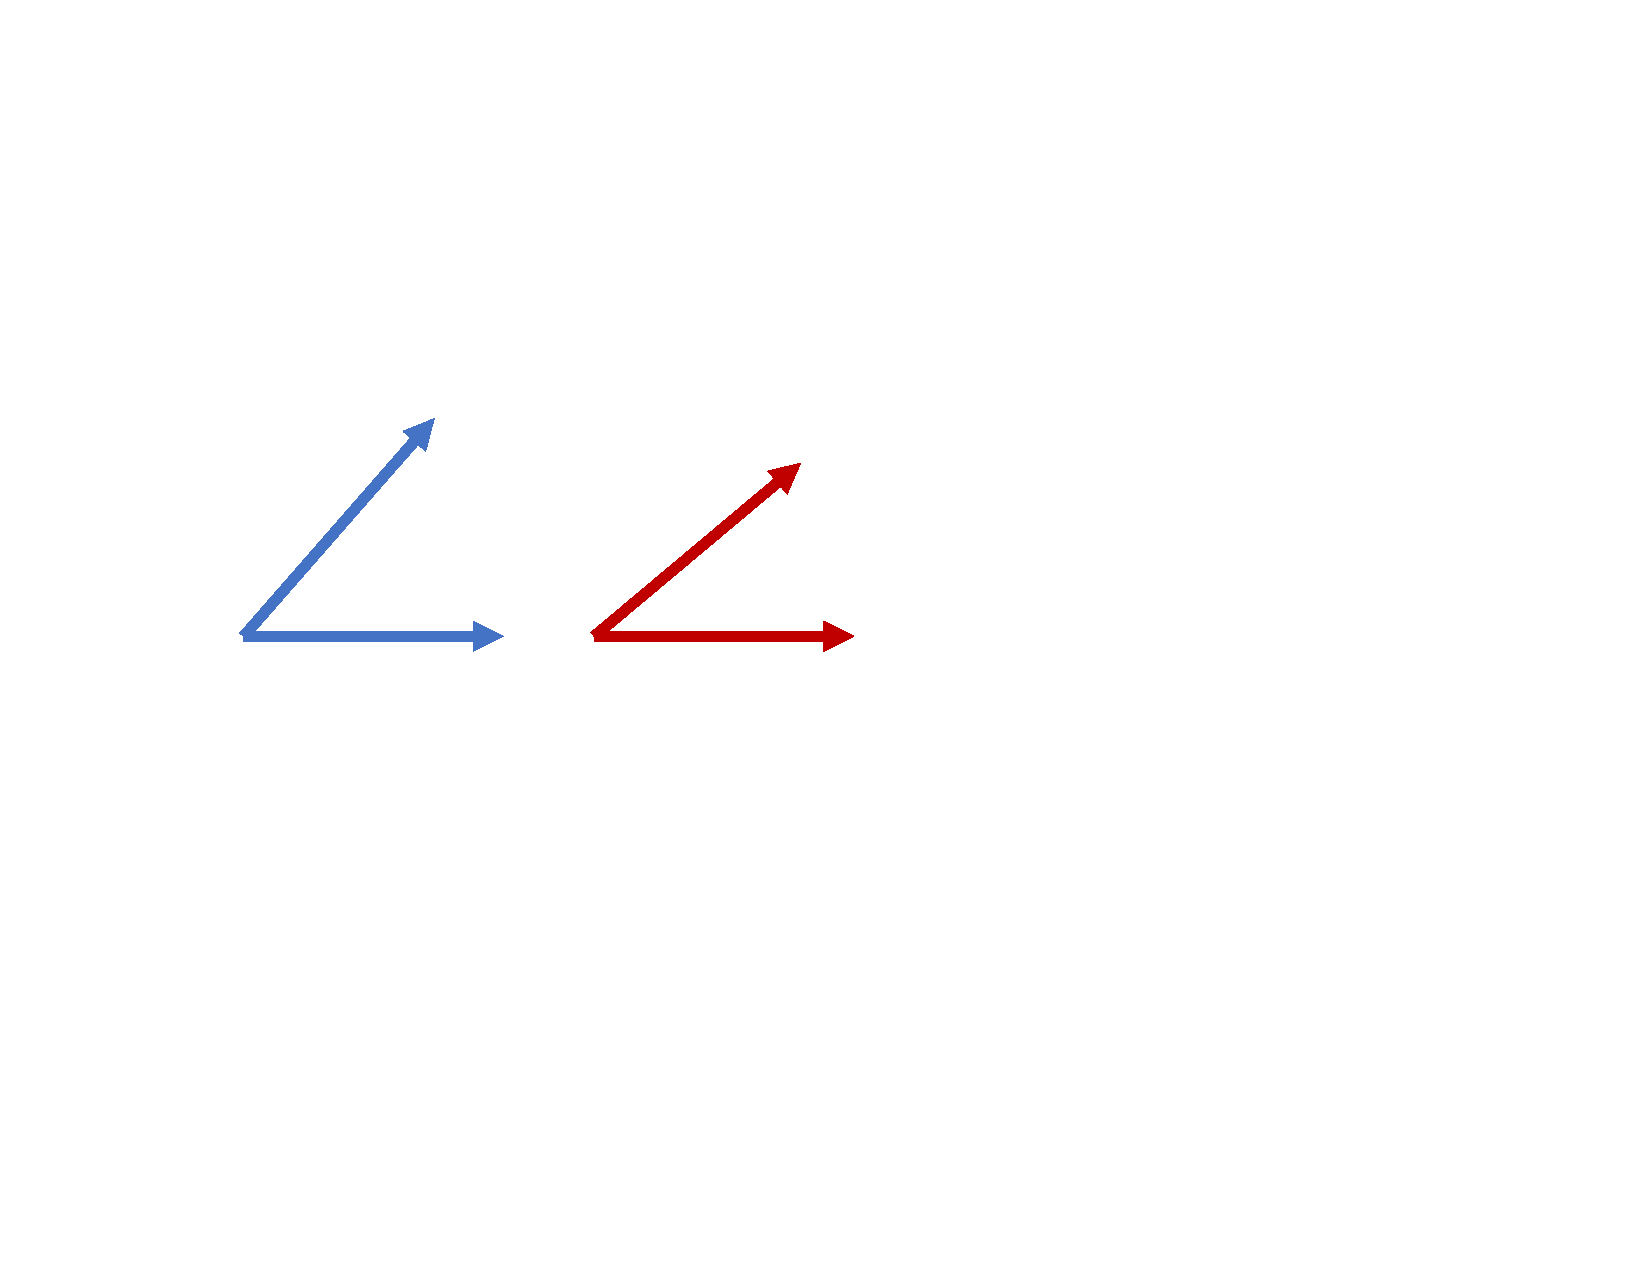
\includegraphics[width=\textwidth, keepaspectratio]{illus/angles.pdf}
    \caption{Illustration of Angles}
    \label{sample_angles}
\end{figure}

\subsection{Experimental Variables and Parameters}

The main variable of interest is diversity bonus, which will be varied at the following values: no diversity bonus $b=1$, which serves as the control; 10\% diversity bonus $b=1.1$ (Treatment 1), and 50\% diversity bonus $b=1.5$ (Treatment 2). With $b=1.1, n_m=7, n_f=3$, there is roughly a 50\% chance that a male candidate is shortlisted. This will ensure that the manager sees an equal number of male and female candidate.

In the theoretical model, recruiters are assumed to shortlist 2 candidates in 2 seperate sub-rounds. Although this assumption makes solving the model tractable, it may not reflect the real world. To address this, an alternate setup is also tested, in which recruiters shortlist 2 candidates in the same round. This is to check whether the empirical results deviate between the two setups.

If resources permit, the proportion of male to female candidates in the initial pool can also be varied.

\begin{center}
    \begin{tabular}{ l l}
        \hline
        Variable                                       & Values    \\
        \hline
        Diversity bonus $b$                            & $1,1.5,2$ \\
        Number of sub-rounds to shortlist 2 candidates & 1,2       \\
        Number of Male/Female candidates               & 3/1,2/2
    \end{tabular}
\end{center}


\subsubsection*{Power Analysis}
Assuming a standard deviation of 0.1, to detect a 10\% effect size of probability that a male is hired with 80\% power at $\alpha=0.05$, we require a sample size of 120 participants in each treatment cell.

\subsection{Data Generating Process}

As mentioned earlier, the candidate's true quality $q$ is composed of 2 components: a deterministic quality score $q'$, which is a function of the candidate's credentials, and a random disturbance term $\epsilon$. $q'$ has a uniform distribution $q' \sim \Unif$. Because the the true quality $q$ also needs to be bounded between 0 and 1, a logit and inverse-logit transform is performed on gaussian noise. This ensures that $q$ is uniformly distributed and bounded between 0 and 1.

$$q_i        = 0.7q'_i + 0.3\epsilon_i$$
$$q_i'= f(\textit{GPA}_i, \textit{Degree}_i, \textit{FieldofStudy}_i, \textit{YrsExp}_i})$$
$$\epsilon_i = \frac{1}{1+ exp(-\mathcal{N}(q'_i, 1))}$$
$$q \sim \Unif$$

\subsection{Estimation}





\end{document}